\documentclass[10pt, a4paper]{article}

% Formatting
\usepackage{ctex}
\usepackage[margin=1in]{geometry}
\usepackage[titletoc,title]{appendix}

\usepackage[colorlinks,linkcolor=red]{hyperref}
\usepackage{amsmath,amsfonts,amssymb,mathtools}


\usepackage{graphicx,float}
\usepackage{xcolor}

\usepackage[ruled,vlined]{algorithm2e}
\usepackage{algorithmic}


\everymath{\displaystyle}


\usepackage{biblatex}
\addbibresource{references.bib}

% Title content
\title{数理统计学习笔记 \par 大作业(一)完成指导}
\author{慕弋云子}
\date{December 4, 2020}

\begin{document}
\maketitle

关于学习笔记的常规内容,可见本文GitHub Repo的地址,在这里你可以找到之前或之后的内容,不会迷路:\url{www.github.com/Muyiyunzi/ShuLiTongJi_BUAA} \par
本文旨在帮助大家事半功倍地完成大作业的相关内容,对于个中原理,我们可以不求甚解(孙老师的八字方针原话:\textbf{点到为止,独立完成}),虽然百度上有一些之前学长学姐的作业,但是毕竟是付费的,大家还得照猫画虎、邯郸学步,排个版也会花费不少的功夫。\par

于是,我在GitHub Repo中上传了.docx的文件,大家可以借此省去排版的功夫,照着这篇文档,也可以“傻瓜式”地快速完成这份大作业。\par
孙老师的原话是,“如果查重率到了七八十,那我可就得处理你了”,所以我的理解是:\textbf{只要数据使用的不同},那些原理什么的抄一抄(注好引用),用软件跑一下得到结果自己分析分析,\textbf{就一定不会被查}。另外孙老师还说,要\textbf{结构完整,敢下判断},所以说除了数据一定要自己找一下之外,剩下的就是按照这篇《完成指导》所给的图去索骥,只要结构完整,就绝对不会为难大家。\par

\section{SPSS的安装}
这个大作业的主要目的是\textbf{让大家学习使用统计软件}。而SPSS这个软件\sout{易于破解,}操作清晰,用于完成大作业简直再合适不过。作为一个六系学生我当然也想过用Python,但想了想研究调库也得有段时间,还是不如SPSS一键生成来得方便。所以在此墙裂推荐大家使用SPSS。\par
我所使用的软件版本是25,各个版本的操作应该都是大同小异,由于我使用的是Windows系统,所以其他系统的童鞋就得自己找一下破解,并跳过本节的剩余内容了。在这里我贴一个Windows系统的度盘链接方便大家直接下载:\href{https://pan.baidu.com/s/1WDLkJQhU631BkLGUSQe1_g}{提取码:beay}。按照下面的指示完成安装和破解。\par
下载后双击运行.exe文件即可,是否安装Python的补充文件、路径等可以自行随缘选择。安装完毕后,不要立即激活,然后将crack.rar解压,将crack目录下的lservrc文件替换到安装目录下。例如我SPSS的安装路径是D:$\backslash$SPSS$\backslash$,那么就将文件复制到这个路径下并选择替换。\par

\begin{figure}[H]
    \centering
    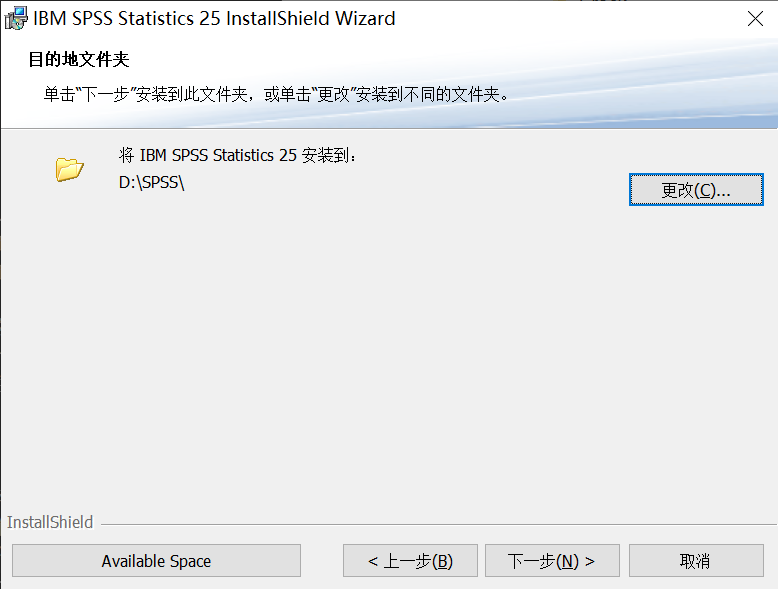
\includegraphics[width=0.7\linewidth]{SPSS.png}
    \caption{IBM SPSS的安装界面}
    \label{fig:SPSS}
\end{figure}

替换完毕后,可以选择使用搜索栏(或Win+S)搜索SPSS,或是在安装路径下打开Stats.exe即可运行SPSS。

\section{数据的选择、处理与查找}

\subsection{数据查找}
这里主要推荐两个地方吧。一个是\href{https://archive.ics.uci.edu/ml/index.php}{UCI Machine Learning Repository},这里面有很多用于机器学习的数据集。点进“View All Dataset”的链接中,左侧的Default Task框框中,有一个Regression,大家可以自行选择数据。
\begin{figure}[H]
    \centering
    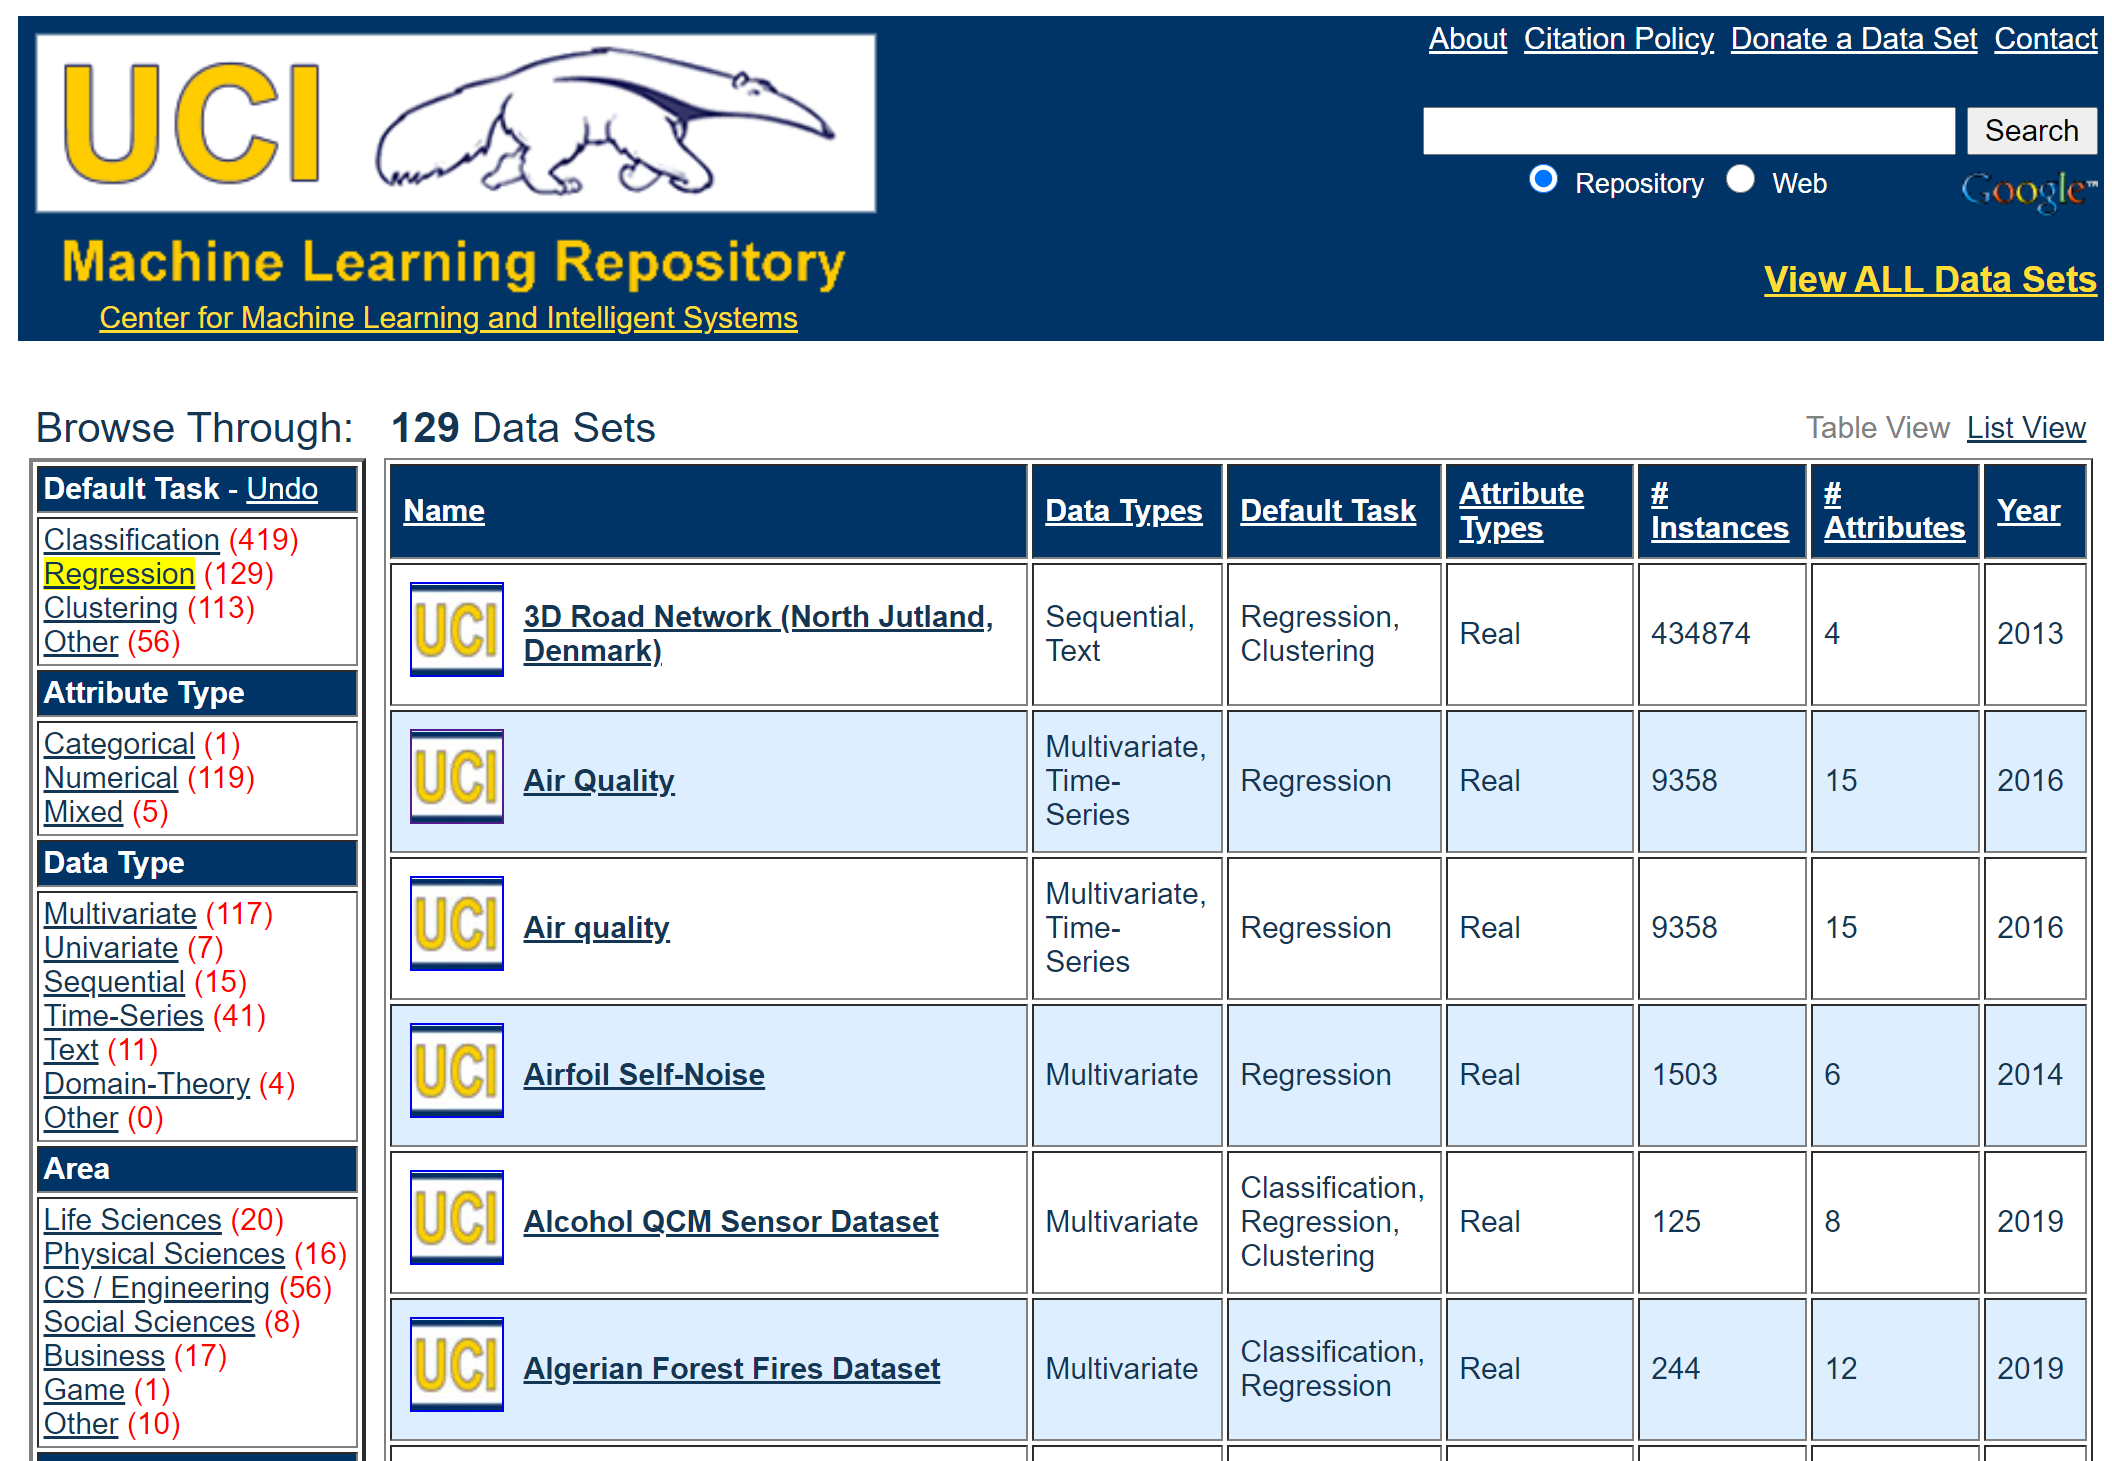
\includegraphics[width=0.7\linewidth]{UCI.png}
    \caption{UCI ML Repo的Regression Task界面}
    \label{fig:UCI}
\end{figure}

再一个就是\href{https://www.datafountain.cn/}{data fountain},在顶部菜单栏处点击数据集即可进行检索。这里面的数据标签大多是汉化过的,不过数据比较杂,可能会有很多非数值特征,使用起来大多需要处理(如何选择和处理见下面两小节)。不过好的是这里面的检索系统还是挺靠谱的,你可以在此检索一些想要的数据,也可以搜索像“价格”、“销售”之类的字眼,会更加利于回归任务。\par

基本上这两个source就可以让大家的数据不重样了。你可别小看这两个数据集,一个Air Quality就能有9000多条数据,你选个100条出来就差不多了,这要是也能有哪位兄弟能跟你选重样了,那可真是……

\subsection{数据选择}
有了数据源,就要学会如何选择,这样才能更好地完成大作业。在数据的选择上,我认为需要注意两点。\par
一、数据一定要是\textbf{数值特征},否则没法做回归。\par
举个例子,我想做笔记本电脑价格的多元线性回归,可以预见到,内存越大、频率越高对价格肯定是正增益的,屏幕分辨率越高、重量越轻、厚度越薄等因素肯定也是正增益的,这些数据都是\textbf{数值的}。这样回归出来的效果好吗?估计是不好的。就算好,也可能回归出来那个常量很大,因为影响电脑的主要因素在于CPU、显卡这些指标,而像i3、i5、i7,AMD还是Intel,6800XT还是3080,这些东西是很难以数值去表示的。如果你的数据集在这些数据上波动很大(比如你拿一个i5的960和一个i9的3080去比,就算他们内存一样、薄厚重量差不多,价位肯定也是天差地别,而你把这些因素忽略掉了),那么回归的效果肯定是不好的,遇到这种情况的话我给两条建议:
\begin{enumerate}
    \item 放弃整个数据集,正所谓there's plenty of fish in the sea,天涯何处无芳草嘛。
    \item 放弃这项非数值特征,反正按照孙老师的说法,点到为止,回归出来线性程度不好就大胆拒绝,有结论就行。
    \item 对这些非数值特征做数值化。比如CPU和GPU的型号可以对应地换成他们在某个benchmark上的评分,然后再去做回归即可,当然了,处理数据会有一些工作量,这就要看你的时间精力,以及对这项工作的喜爱程度了。
\end{enumerate} \par
二、数据要尽量有实际意义,一是方便你写论文,二也算是让自己做的东西有些意义。\par
这是一个数据量爆炸的时代,但并不一定所有数据都有用。比如我手头有近些年英国足球超级联赛的数据,我该怎么入手分析呢?也就是一个核心的问题:如何确定因变量,以及\textbf{回归到底有什么用?}这才是这个大作业需要把握的核心问题。\par
我认为,回归就是为了确定是不是线性关系,以及能够为将来的数据做出预测。\par
比如射门数对于进球数的贡献是不是线性增益?是我射门数越多进球概率就会越大,还是说呈指数性地,我就算射几十上百次也不一定进的了几个球,这是「确定线性关系」。\par
如果我做完回归后,得到了进球数与射门数、角球数、犯规数等诸多指标的线性拟合式,我作为一个教练是不是就可以更好地布置战术,比如犯规对进球数是正增益我就要多让球员犯规;我作为一个赌狗,是不是就可以更好地根据比赛数据预测比赛结果,进行相应地投注指导;我作为一个显卡爱好者,是不是就可以根据这些计算单元数量、吞吐量等指标来预测显卡“香不香”,这些都是所谓「预测」。\par
带着这些目的,就可以更好地选择数据和选择相关变量,至于你要确定什么关系,要做何种预测,就是自己的事情了。

\subsection{数据处理}
这里的数据处理主要是针对于非数值特征而言的。我建议大家使用excel去处理数据,还是比较便捷的,使用一些基本的逻辑语句即可。在这里我以我自己的大作业为例,教大家一些简单的数据处理方法(如果不需要处理,或excel技巧高超,此节内容跳过即可)。\par
比如以下是我拿到的原始数据:
\begin{figure}[H]
    \centering
    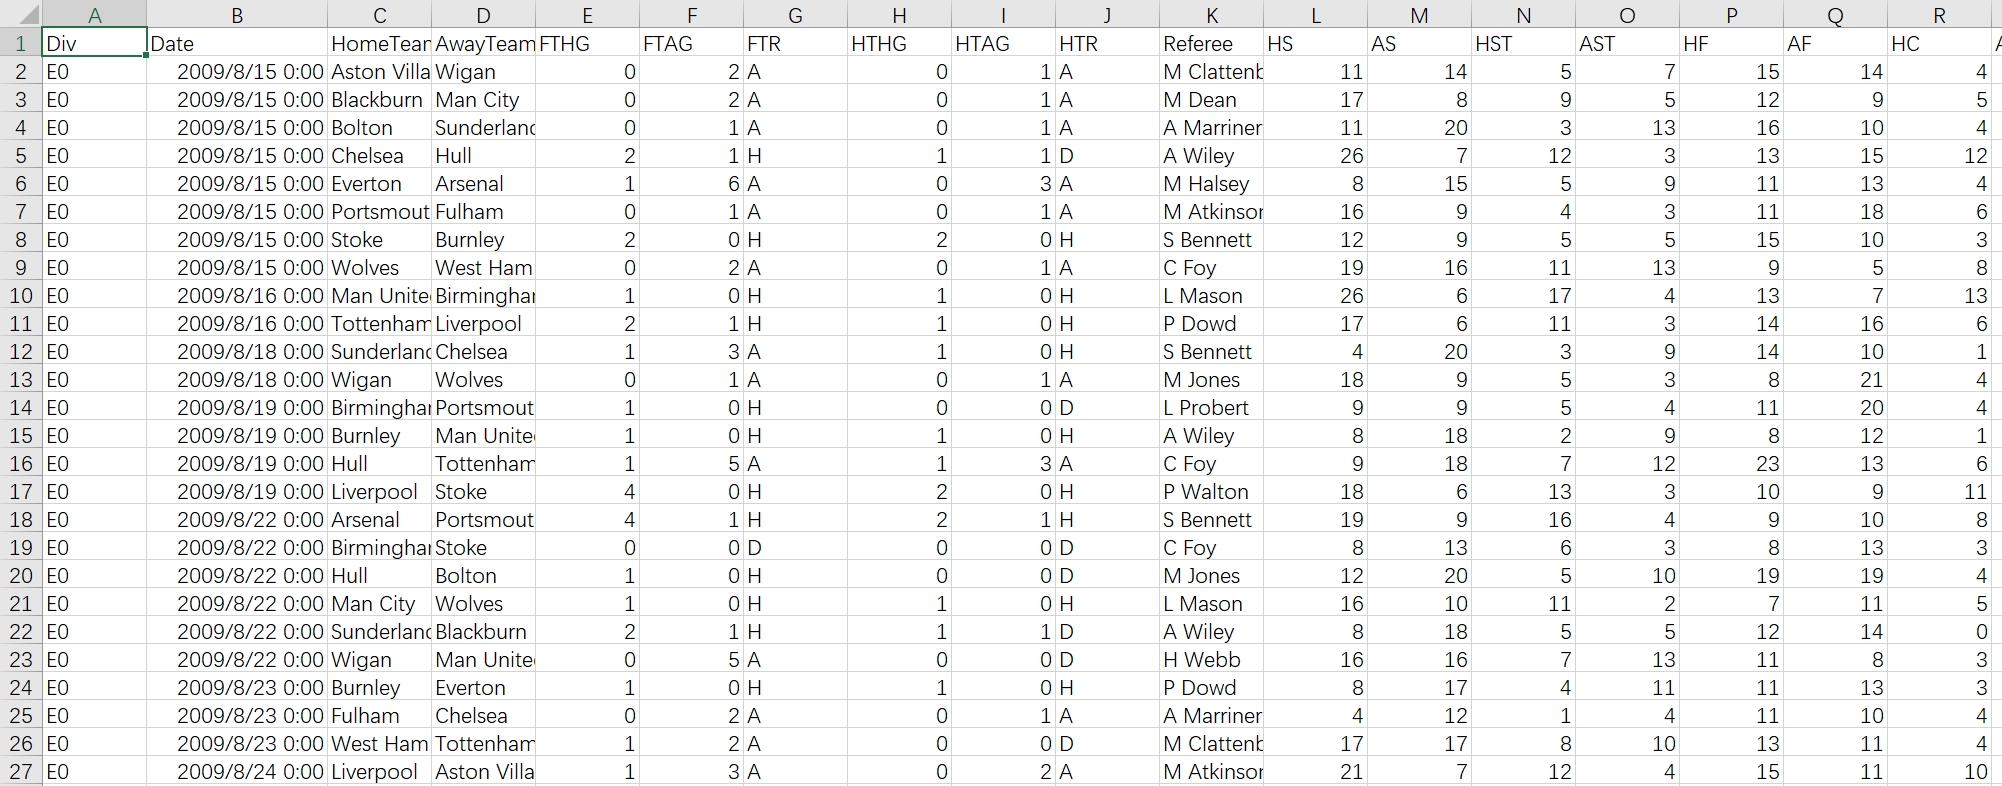
\includegraphics[width=\linewidth]{raw.png}
    \caption{原始数据}
    \label{fig:raw}
\end{figure}\par

原始的数据是从data fountain上获取的(去查了原始网站),是每轮比赛的对阵情况,以及对应的一些比赛数据。那么首先要做的就是去除冗余信息,比如每轮的对阵情况太过杂乱,要么我就单取出几轮,去分析整个联赛的情况;要么我就单独取出一支队伍,然后去考察这支队伍的情况。\par
这里我是通过查找操作,手工高亮出某支球队(Arsenal)的比赛数据(毕竟一个赛季也就38场,我觉得手工操作量不大)。然后将这些英文的特征对应原始网站提供的notes.text(大部分数据集也都会提供类似的说明文件)汉化一下,并去除冗余信息后大概是这个样子:
\begin{figure}[H]
    \centering
    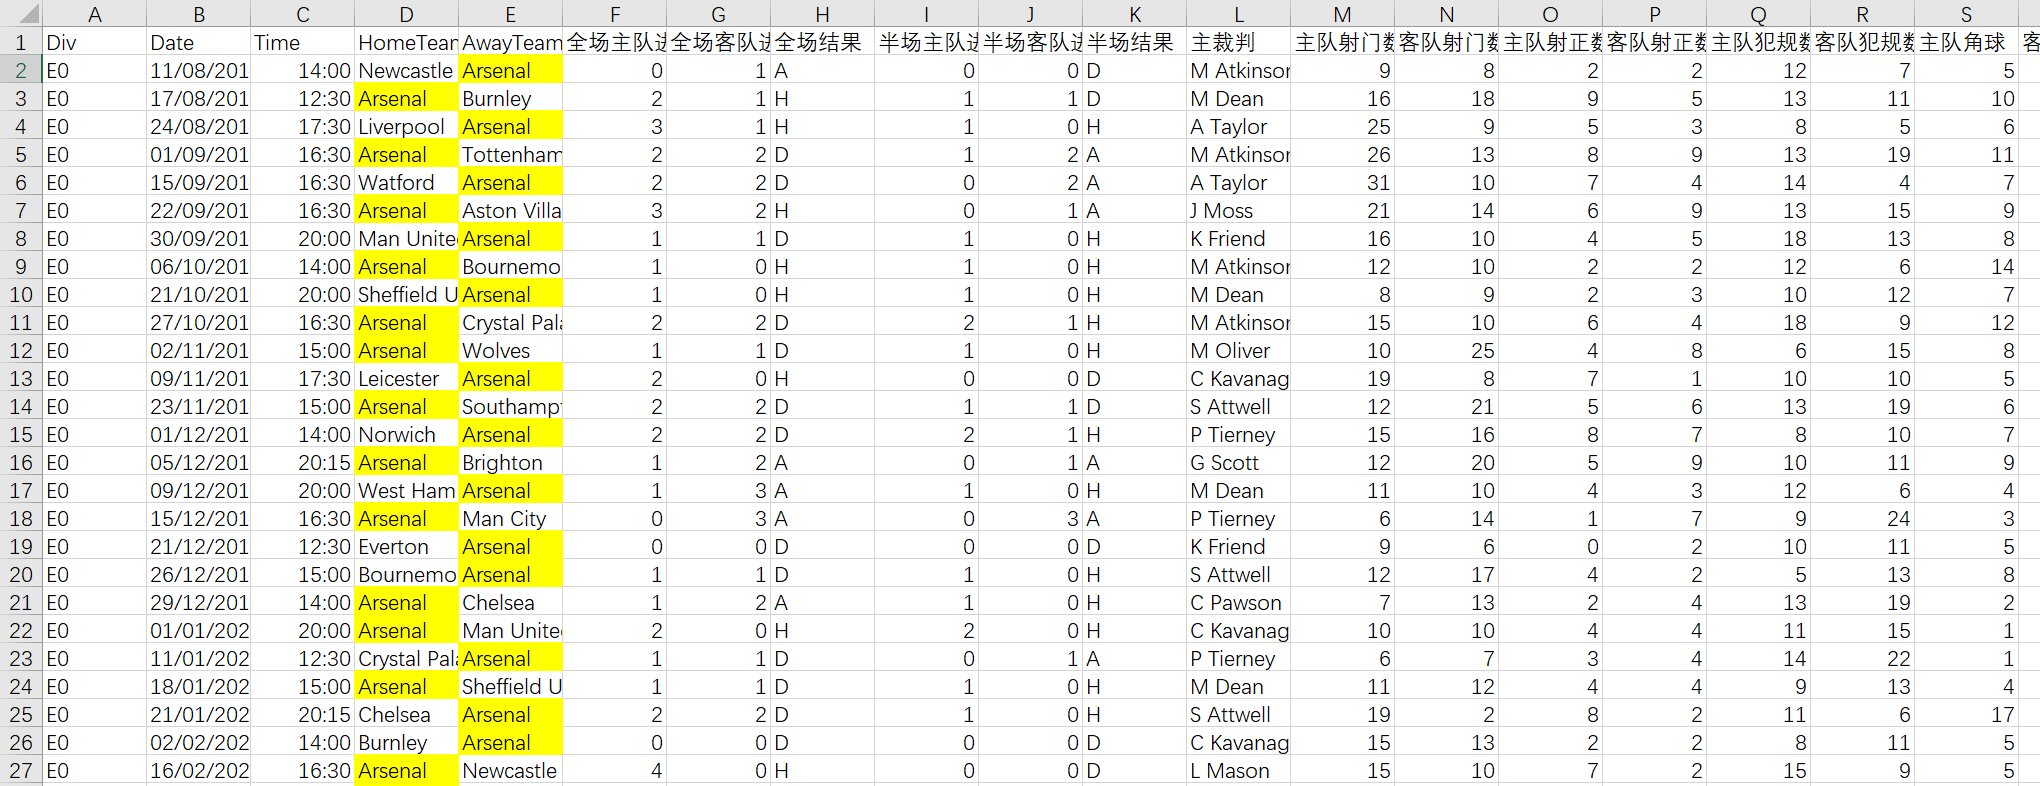
\includegraphics[width=\linewidth]{first.png}
    \caption{初步去除后}
    \label{fig:first}
\end{figure}\par
根据我作为一个足球狗的先验知识,客场作战肯定影响很大,我不想放弃掉这一信息,所以就单开了一栏表示是否客场。这里我将这个非数值特征二值化了——虽然武断了些,但也有好处:如果我们将客场以1表示,主场以0表示,那么最后分析出来的那个系数就应该是直接增益!倘若我的因变量是胜率,那么最后就能直接回归出,如果是客场就可以直接带来多少的胜率增加/减少,这是非常直观的。\par
这里可以使用Excel中的IF逻辑判断。选中某一个块,在其上输入判断语句:
\begin{center}
    =IF(E2="Arsenal",1,0)
\end{center}
其中IF语句的第一个分量表示判断条件,第二个分量为判断为真时此块的value,第三个分量为判断为假时的value(多说一句,所以这其实是个三目表达式啊),这里E2表示E列的第二个块,在我的数据中表示客场的球队。\par

\begin{figure}[H]
    \centering
    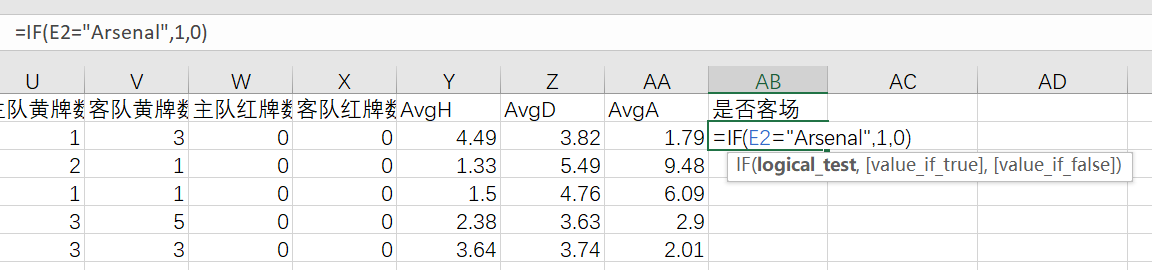
\includegraphics[width=0.9\linewidth]{IF.png}
    \caption{IF语句的使用}
    \label{fig:IF}
\end{figure}\par
如果一切顺利的话,就会输出1或者0,接下来要做的就是大家在Excel中都会的,将鼠标指针放到块的右下角,变成加号后按住左键往下拉,就可以神奇地自动逐行生成判断了。由此,我们便完成了将一个非数值特征二值化的操作。\par
此后还有一些对数据的运算,基本就是在Excel中敲公式了,如果不会敲公式的话,可以去查阅我的大作业以及文件夹中的.xlsx文件,在此不再赘述。\par
再就是尽量选一些数字大的东西去回归(比如胜率能用$50\%$就不用$0.5$),这样回归出来的系数不至于太难看。就像我也放弃了进球数作为因变量,而是用博彩胜率这样一个阈值更大的数据作为因变量。\par
由此我们便得到了最终的数据:

\begin{figure}[H]
    \centering
    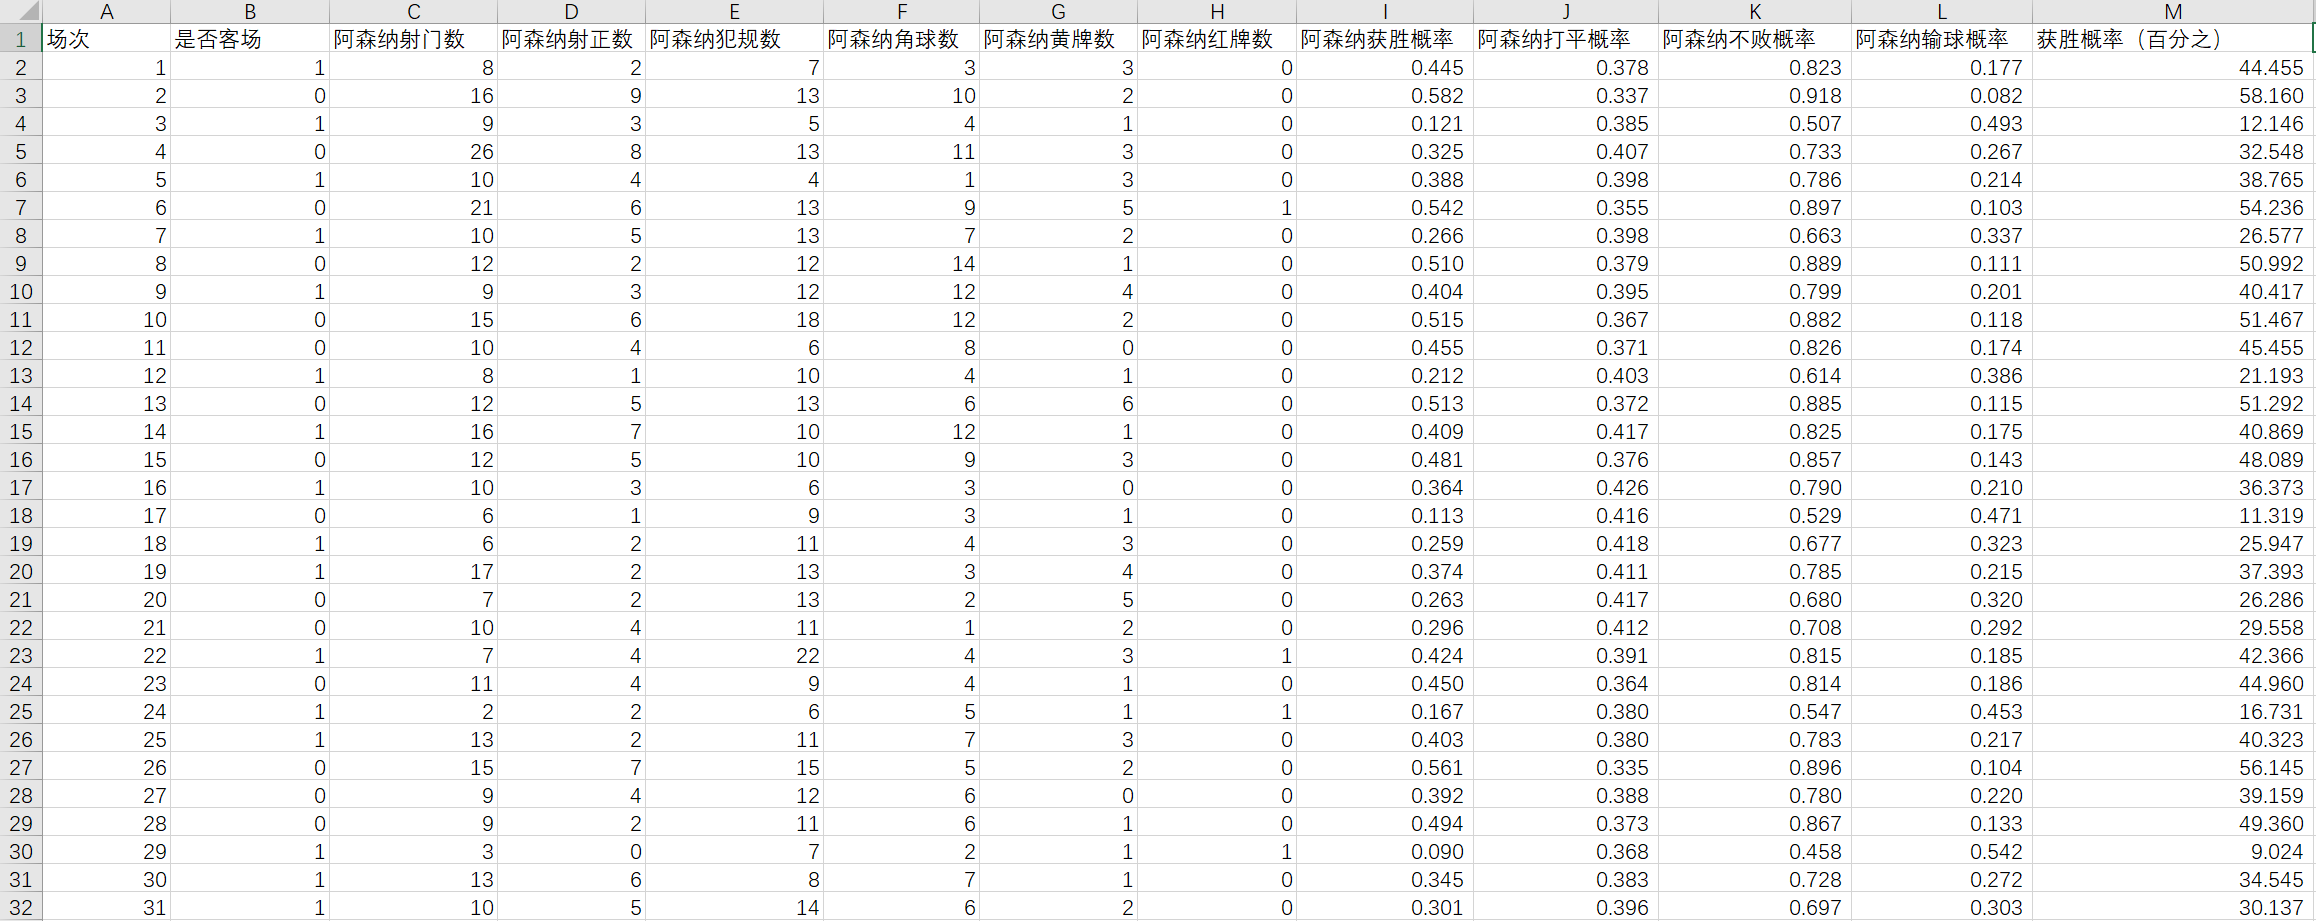
\includegraphics[width=\linewidth]{final.png}
    \caption{最终数据}
    \label{fig:final}
\end{figure}\par

其中打平、不败、输球这三栏数据我是做备用的,如果胜率做因变量的效果不好,可以换这些试试。

\section{使用SPSS完成回归任务}
将最终数据存好在.xls/.xlsx文档之后,便可以导入SPSS完成回归任务了。这里有许多细节需要注意,我在这里先给出完整的操作,再补充解释。
\begin{enumerate}
    \item 导入数据,可以通过欢迎页的打开导入,也可以通过菜单栏的文件->打开->数据打开,只是注意要在文件类型处选择excel表格,才能找到你的数据。
    \begin{figure}[H]
        \centering
        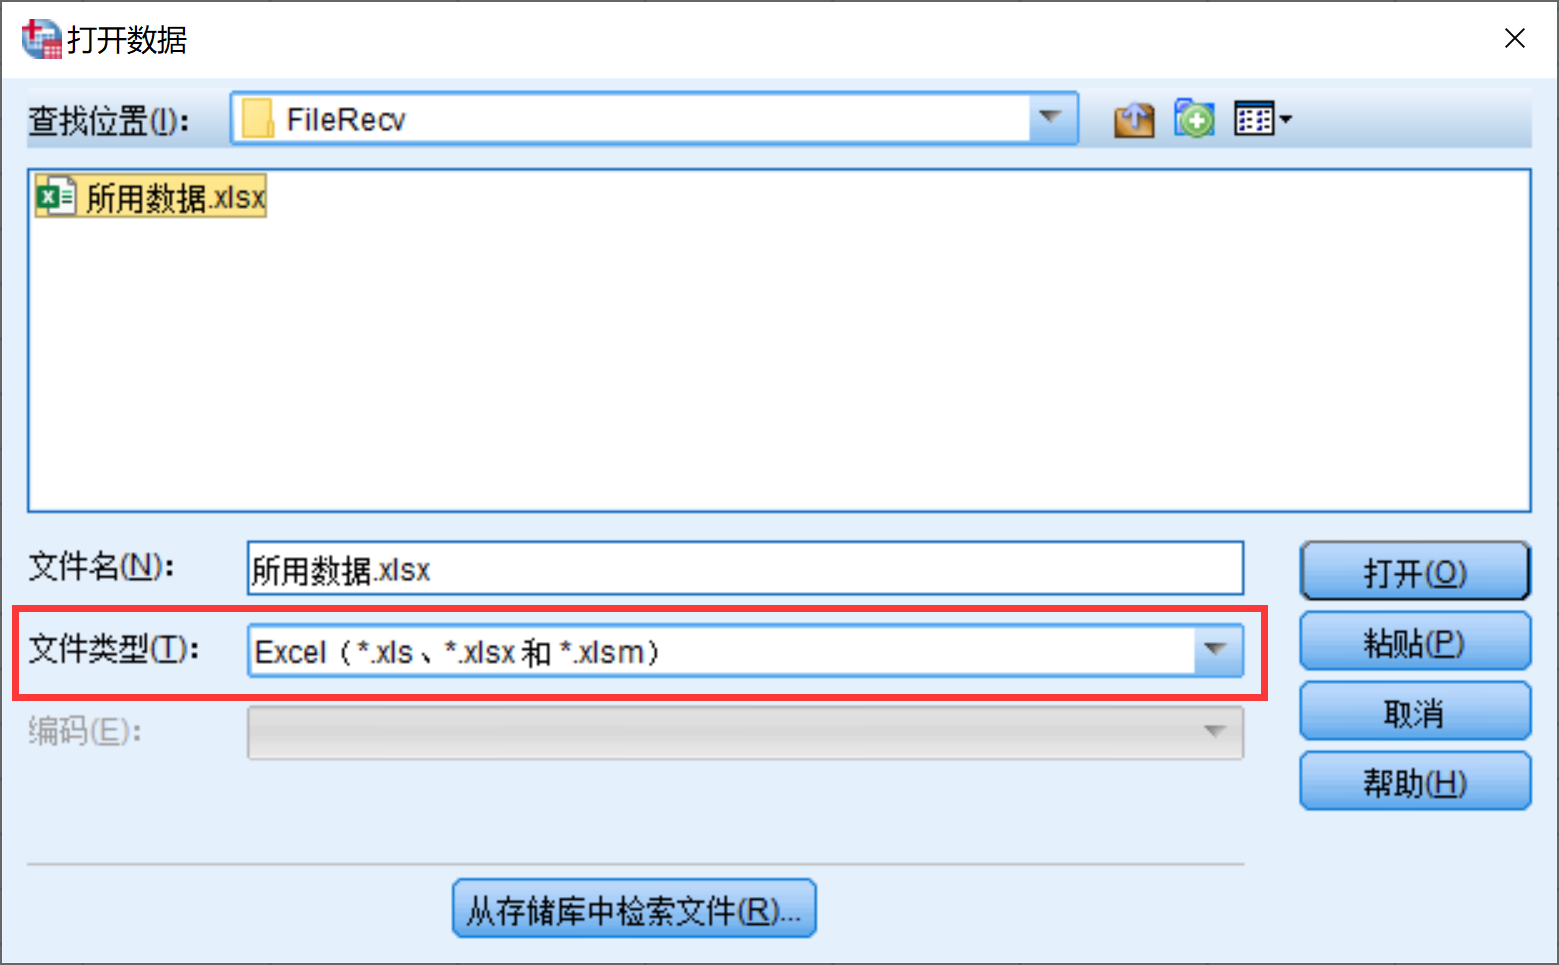
\includegraphics[width=0.5\linewidth]{import.png}
        \caption{导入数据}
        \label{fig:import}
    \end{figure}
    \item 点击打开后会弹出一个对话框。如果工作表有多个sheet,选择你使用数据的那个sheet;然后默认会有三个tick,第二个tick“用于确定……”建议反选掉,虽然选上好像也没啥事儿。然后点击确定。
    \item 这时应该会看到数据被导入。在菜单栏选择:分析->回归->线性,会弹出一个对话框,此时将因变量选中,点击添加按钮添加到因变量区域,再选中自变量,然后添加到自变量区域,如下图所示。友情提示,这里选中自变量的时候可以巧用shift或者ctrl操作,不用一个个点。
    \begin{figure}[H]
        \centering
        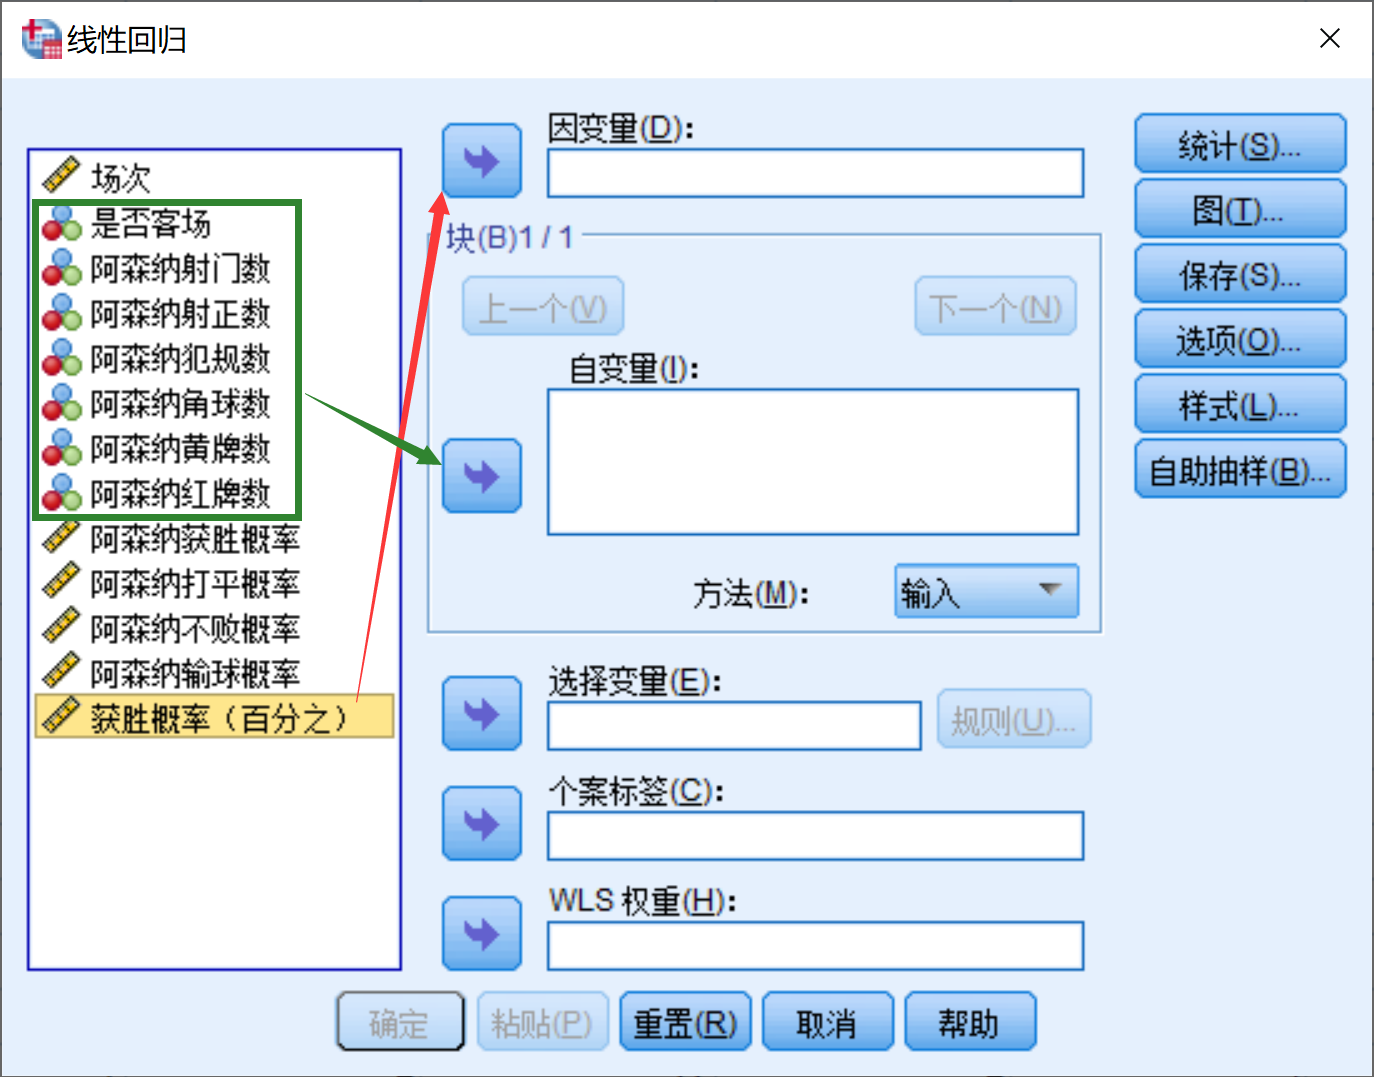
\includegraphics[width=0.5\linewidth]{select.png}
        \caption{选择变量}
        \label{fig:select}
    \end{figure}
    \item 将方法从默认的「输入」改成「步进」,这样就是逐步回归法了。
    \item 随后点击「图」按钮,勾选标准化残差图区域中的两个框框,这东西用于分析数据的正态性。
    \begin{figure}[H]
        \centering
        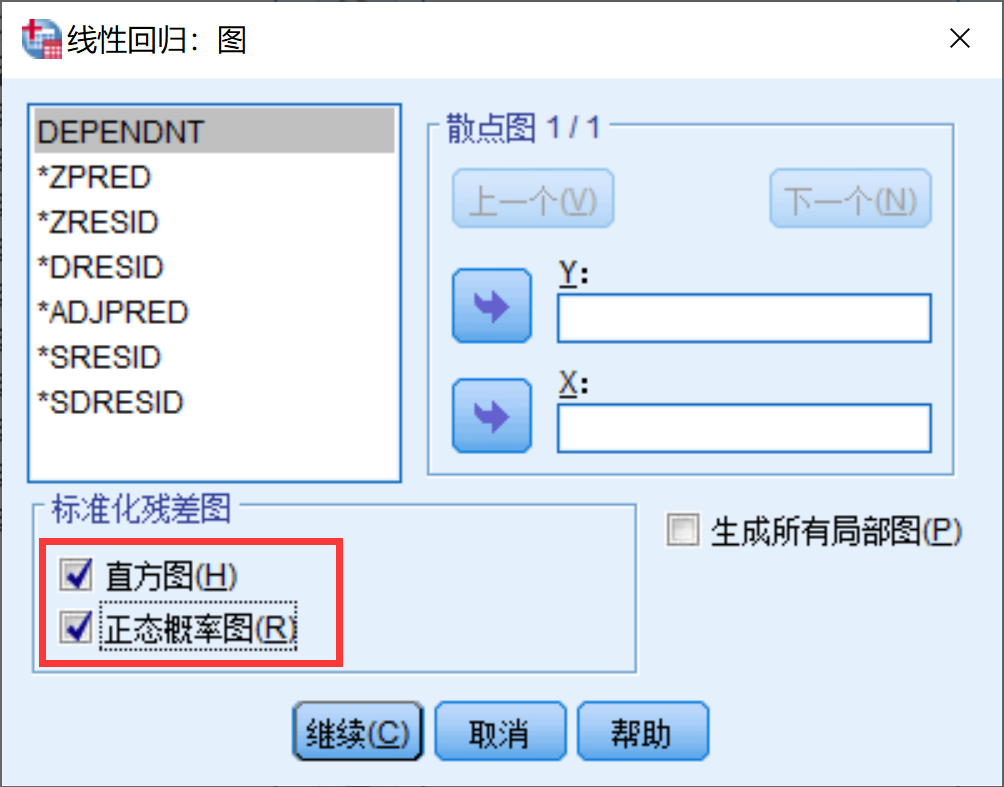
\includegraphics[width=0.3\linewidth]{graph.png}
        \caption{「图」按钮对话框}
        \label{fig:graph}
    \end{figure}
    \item 继续后点击「选项」按钮,“使用F的概率”那一条中,可以自己设置进入和除去值。一般来讲0.05和0.10的组合都得不出啥结论,可以调成0.2+0.25或是0.4+0.5的组合分别看看效果,都试试。
    \begin{figure}[H]
        \centering
        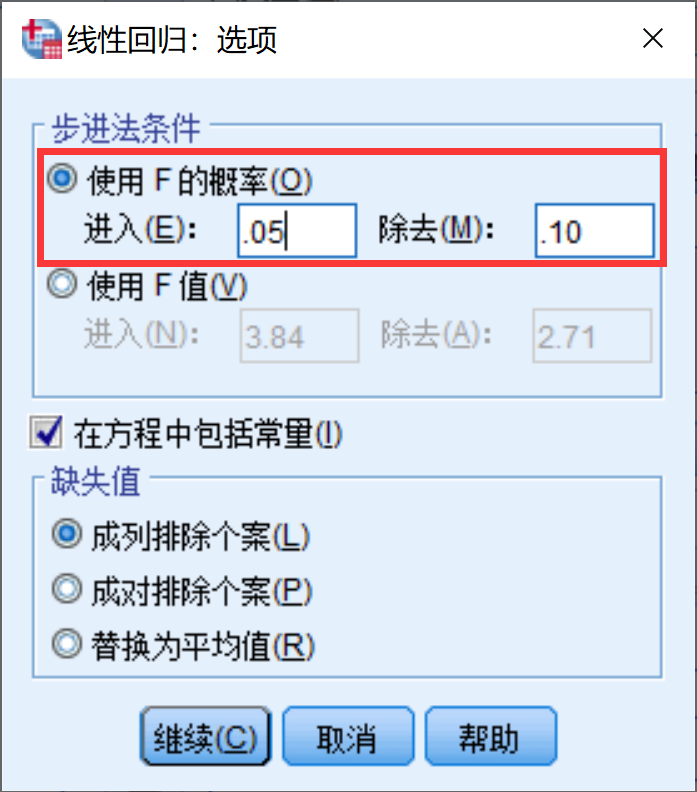
\includegraphics[width=0.3\linewidth]{stepwise.png}
        \caption{「选项」按钮对话框}
        \label{fig:stepwise}
    \end{figure}
    \item 其余选项都默认不要管,然后确定,即可生成各个表格。
    \item 接下来要做的就是把这些表格对应地替换报告模板中的表格即可。
\end{enumerate} \par
这里稍微对分析结果进行解释一下。
\begin{enumerate}
    \item 输入/除去的变量中,表示了在你设置的这个F值组合中,按照显著性的程度,步进获得的变量。也就是说表格中越靠上的变量显著性越小(置信度越高)。另外就是,通常来讲是没有除去变量的。
    \item 根据输入/除去的变量顺序,因为其逐步性,可以分别得到几个模型,这些模型都记录在了模型摘要表中。
    \item ANOVA不用太在意,照搬即可,一般就看最后那个显著性一栏,不太离谱就行。
    \item 系数表比较重要,你最终会选择其中一个模型作为最优模型(你看着选,毕竟点到为止,有结构就行),那么最终多元回归的表达式就应该是$y=b+\sum c_i x_i$的形式,这里的$c_i$就都在这张表里了。你的报告里也应该有对应的完整表达式。
    \item 系数表的显著性其实比较重要,一般来讲要小于0.05才算是比较能接受模型,但是你也得多点变量嘛,所以这里可以睁一只眼闭一只眼。
    \item 排出的变量这张表没啥好说的,我认为不用贴;参差统计和后面的两个正态性的图都要贴上去,这可是老师点名要的图。
\end{enumerate}

\section{完成报告}
这一部分相信大家可以照葫芦画瓢完成,应该没什么太多要说的。至于报告各部分的内容,韦老师和孙老师班的要求略有差异,但我认为我这样对于两个班的要求来讲应该都是ok的,大家还是要把重心放在学习知识和考试上,大作业这种东西,大家体验体验就是了哈哈哈。\par
格式方面,我在上传的.docx报告文件中也调整了样式库,大家如果需要自行加标题的话记得选样式、敲公式的话记得选公式样式然后使用制表位,参考文献换行会自动生成编号,最后也别忘了更新目录。\par
内容方面,大家在替换表格的时候可以从SPSS中复制,然后粘贴的时候选择保留源格式,然后选中后设置居中及边框全满,大概看起来会好看些吧。总之这些大家随意吧,原理的那些死的东西也都不用改,涉及数据和分析的活的东西要自己写一写,大概就是这样,如有任何问题欢迎在GitHub上提Issue,我会随缘解答。

\end{document}